%!tikz editor 1.0
%!tikz source begin
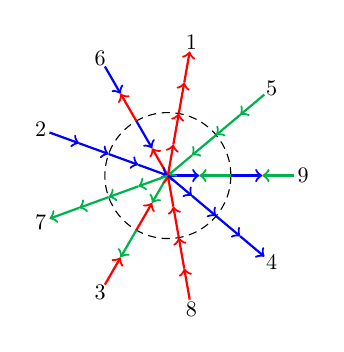
\begin{tikzpicture}[scale=.4,every node/.style={scale=.8}]

	%% Settings
	\pgfmathsetmacro{\Nutzahl}{9}

	\pgfmathsetmacro{\winkel}{360/\Nutzahl}

	\tikzstyle{outside}=[->, thick]
	\tikzstyle{inside}=[<-, thick]
	
	\draw[densely dashed] (0,0) circle (2);
	
	\foreach \i in {1,2,...,\Nutzahl}
	{	
		\node at (2*\i*\winkel:4.3) {\i};		
	}

	\begin{scope} [rotate=(0)*\winkel]
		\draw [color=blue, outside] (0:0) -- (0:1);
		\draw [color=green!70!blue, inside] (0:1) -- (0:2);
		\draw [color=blue, outside] (0:2) -- (0:3);
		\draw [color=green!70!blue, inside] (0:3) -- (0:4);
	\end{scope}

	\begin{scope} [rotate=(1)*\winkel]
		\draw [color=green!70!blue, inside] (0:0) -- (0:1);
		\draw [color=green!70!blue, inside] (0:1) -- (0:2);
		\draw [color=green!70!blue, inside] (0:2) -- (0:3);
		\draw [color=green!70!blue, inside] (0:3) -- (0:4);
	\end{scope}

	\begin{scope} [rotate=(2)*\winkel]
		\draw [color=red, outside] (0:0) -- (0:1);
		\draw [color=red, outside] (0:1) -- (0:2);
		\draw [color=red, outside] (0:2) -- (0:3);
		\draw [color=red, outside] (0:3) -- (0:4);
	\end{scope}

	\begin{scope} [rotate=(3)*\winkel]
		\draw [color=red, outside] (0:0) -- (0:1);
		\draw [color=blue, inside] (0:1) -- (0:2);
		\draw [color=red, outside] (0:2) -- (0:3);
		\draw [color=blue, inside] (0:3) -- (0:4);
	\end{scope}

	\begin{scope} [rotate=(4)*\winkel]
		\draw [color=blue, inside] (0:0) -- (0:1);
		\draw [color=blue, inside] (0:1) -- (0:2);
		\draw [color=blue, inside] (0:2) -- (0:3);
		\draw [color=blue, inside] (0:3) -- (0:4);
	\end{scope}

	\begin{scope} [rotate=(5)*\winkel]
		\draw [color=green!70!blue, outside] (0:0) -- (0:1);
		\draw [color=green!70!blue, outside] (0:1) -- (0:2);
		\draw [color=green!70!blue, outside] (0:2) -- (0:3);
		\draw [color=green!70!blue, outside] (0:3) -- (0:4);
	\end{scope}

	\begin{scope} [rotate=(6)*\winkel]
		\draw [color=green!70!blue, outside] (0:0) -- (0:1);
		\draw [color=red, inside] (0:1) -- (0:2);
		\draw [color=green!70!blue, outside] (0:2) -- (0:3);
		\draw [color=red, inside] (0:3) -- (0:4);
	\end{scope}

	\begin{scope} [rotate=(7)*\winkel]
		\draw [color=red, inside] (0:0) -- (0:1);
		\draw [color=red, inside] (0:1) -- (0:2);
		\draw [color=red, inside] (0:2) -- (0:3);
		\draw [color=red, inside] (0:3) -- (0:4);
	\end{scope}

	\begin{scope} [rotate=(8)*\winkel]
		\draw [color=blue, outside] (0:0) -- (0:1);
		\draw [color=blue, outside] (0:1) -- (0:2);
		\draw [color=blue, outside] (0:2) -- (0:3);
		\draw [color=blue, outside] (0:3) -- (0:4);
	\end{scope}

\end{tikzpicture}
%!tikz source end
